\documentclass[11pt,twoside,openright]{book}

% =============================================================================
% Mass Spectrometry Data Analysis with R
% Chapter 21: Differential Abundance Analysis Using Linear Models & Empirical Bayes
% Author: Lucas VHH TRAN (CK-CARE Davos)
% Style: Springer Nature Monograph (Health Analytics with R Pedagogy)
% =============================================================================

\usepackage{springer_monograph}

\hypersetup{
    pdftitle={Chapter 21: Differential Abundance Analysis Using Linear Models and Empirical Bayes Moderation},
    pdfauthor={Lucas VHH TRAN}
}

\begin{document}

\setcounter{chapter}{20}
\chapter{Differential Abundance Analysis Using Linear Models and Empirical Bayes Moderation}

\noindent
\textbf{Lucas VHH TRAN}\footnote{CK-CARE Davos, Christine K\"uhne -- Center for Allergy Research and Education, Davos, Switzerland. Email: \texttt{lucas.tran@ck-care.ch}}\\
\rule{\textwidth}{0.8pt}

\begin{abstract}
\noindent
Differential abundance analysis constitutes the central inferential milestone in quantitative mass spectrometry (MS), bridging upstream peptide identification, feature extraction, and normalization with downstream biological pathway interpretation. In bottom-up proteomics and untargeted metabolomics, thousands of biomolecular entities ($p \approx 10^3$--$10^4$) are profiled across a limited cohort of biological replicates ($n \approx 3$--$10$ per phenotype). Under such severe small-sample high-dimensional regimes ($p \gg n$), conventional statistical tests (e.g., standard Student's $t$-tests and ordinary ANOVA) suffer catastrophic loss of statistical power and variance instability: features with underestimated sample variances yield spuriously inflated test statistics, manufacturing hundreds of false-positive discoveries out of measurement noise. 

This chapter develops the theoretical, mathematical, and practical foundations of empirical Bayes variance moderation pioneered by Gordon Smyth (\texttt{limma}) and adapted for quantitative mass spectrometry. We formulate the high-dimensional linear regression framework, explicate the inverse-gamma prior distribution for feature-specific error variances, derive the closed-form moderated $t$-statistic and log-odds ($B$-statistic), and establish rigorous false discovery rate (FDR) control via the Benjamini--Hochberg and Storey procedures. We provide complete algebraic formulations for two-group, factorial, paired, and multi-site blocked designs. The methodology is operationalized through a hands-on, step-by-step computational R laboratory utilizing the benchmark 11-site Data-Independent Acquisition (DIA) multi-laboratory reproducibility study (PXD004886) containing synthetic AQUA spike-in positive controls. The chapter concludes with an audit of the ten deadly sins of differential omics, comprehensive multi-tier exercises, and fully worked-out step-by-step mathematical and algorithmic solutions.
\end{abstract}

\noindent
\textbf{Keywords:} Differential Abundance, Empirical Bayes, Linear Models, \texttt{limma}, False Discovery Rate, Mass Spectrometry, Proteomics, Volcano Plot, Contrast Matrix.

\vspace{0.8em}
\noindent\rule{\textwidth}{0.4pt}

% =============================================================================
% Tutor's Methodological Roadmap
% =============================================================================

\begin{table}[ht]
\centering
\caption{Tutor's Methodological Roadmap: Four Checkpoints for Differential Abundance Analysis}
\label{tab:diff_roadmap}
\small
\begin{tabularx}{\textwidth}{l p{3.8cm} p{4.2cm} X}
\toprule
\textbf{Stage} & \textbf{Physical Mechanism} & \textbf{Key Analytical Objective} & \textbf{Primary Failure Mode \& Remedy} \\
\midrule
\textbf{1. Linear Model} & Small sample size ($n \approx 3$--$5$ per group); multi-factor experimental layouts \cite{smyth2004linear, ritchie2015limma}. & Formulate design matrix $\mathbf{X}$ and contrast vectors $\mathbf{c}^T \boldsymbol{\beta}$ for target biological hypotheses. & Mis-specifying factorial designs or omitting batch blocks. Remedy: Use group-means parameterization \cite{law2014voom}. \\
\addlinespace
\textbf{2. Variance Shrinkage} & Erratic small-sample variances ($d_g = 4$); high noise in low-abundance ions \cite{karpievitch2012statistical, lazar2016accounting}. & Shrink feature variances toward prior $s_0^2$ with $d_0$ degrees of freedom; compute moderated $\tilde{t}_g$. & Using unmoderated $t$-tests ($40\%$ false discovery rate). Remedy: Empirical Bayes moderation via \texttt{eBayes} \cite{smyth2004linear, phipson2016robust}. \\
\addlinespace
\textbf{3. Multiple Testing} & High-dimensional hypothesis testing ($p \approx 10^3$--$10^4$ simultaneous tests) \cite{benjamini1995controlling, storey2003statistical}. & Control False Discovery Rate (FDR) via Benjamini--Hochberg step-up or Storey $q$-values ($\alpha = 0.05$). & Reporting uncorrected $p$-values. Remedy: Apply Benjamini--Hochberg adjustment and inspect $p$-value histograms \cite{efron2004large}. \\
\addlinespace
\textbf{4. Missingness \& Robustness} & Left-censored MNAR values in low-abundance peptides; outlier ion scans \cite{ahlmann2020proda, goeminne2016msqrob2}. & Deploy probabilistic dropout modeling (\texttt{proDA}) or robust Huber/Tukey regression. & Naive global imputation creating synthetic fold changes. Remedy: Model missingness directly \cite{choi2014msstats}. \\
\bottomrule
\end{tabularx}
\end{table}

\begin{notebox}
\textbf{Tutor's Methodological Advice: The Degrees of Freedom Axiom}\\
In high-throughput mass spectrometry experiments with $n = 3$ replicates per group, the ordinary residual degrees of freedom is only $d_g = 6 - 2 = 4$. With so few degrees of freedom, the sample variance $s_g^2$ is an extremely volatile estimator of true variance $\sigma_g^2$. Ordinary $t$-tests divide by near-zero sample variances, producing massive test statistics for purely uninformative noise. Smyth's empirical Bayes moderation augments the effective degrees of freedom to $d_g + d_0$, where $d_0$ reflects information borrowed across all $5{,}000$ proteins in the experiment. Never execute an unmoderated $t$-test on small-cohort omics data \cite{smyth2004linear, ritchie2015limma}.
\end{notebox}


% =============================================================================
\section{The Importance of Differential Abundance in Mass Spectrometry}
% =============================================================================

High-throughput mass spectrometry measures the relative or absolute abundance of thousands of proteins, peptides, or metabolites across biological states \cite{aebersold2016mass, cox2008maxquant, demichev2020dia, gatto2023qfeatures}. Whether interrogating a cancer biopsy cohort, a drug-treatment time course, or microbial adaptations to nutrient deprivation, the primary analytical objective is almost universally comparative: \textit{Which molecular entities undergo statistically genuine, biologically meaningful changes in abundance between phenotypic conditions?}

In classical univariate statistics, testing the equality of two population means $\mu_1 = \mu_2$ relies on Student's two-sample $t$-test. In modern omics, however, the analyst faces four physical and statistical realities inherent to mass spectrometry:

\begin{enumerate}
    \item \textbf{The High-Dimensional Small-Sample Regime ($p \gg n$):} Modern LC-MS/MS platforms routinely quantify $5,000$ to $10,000$ protein groups or $1,000$ to $3,000$ metabolite features across only $3$ to $5$ biological replicates per group \cite{navarro2016multicenter}. With $d_g = 4$ residual degrees of freedom, sample variance estimates fluctuate erratically across several orders of magnitude purely by sampling error \cite{smyth2004linear, ritchie2015limma}.
    \item \textbf{Dynamic Range and Mean-Variance Dependence:} MS ion intensities span five to six orders of magnitude ($10^3$ to $10^9$). Lower-abundance features exhibit higher technical coefficients of variation (CV) and elevated rates of missingness (Missing Not At Random, MNAR), whereas high-abundance housekeeping proteins display lower variance \cite{karpievitch2012statistical, lazar2016accounting}.
    \item \textbf{Multi-Layered Batch and Nuisance Structure:} Instrument drift, column maintenance, electrospray emitter fouling, and multi-day digestions introduce technical variance that frequently eclipses subtle biological signals unless explicit blocking factors or pairing constraints are incorporated into the design matrix \cite{johnson2007adjusting, leek2010tackling}.
    \item \textbf{Multiplicity and the Multiple Comparison Problem:} Testing $5,000$ proteins simultaneously at an unadjusted $\alpha = 0.05$ expects $250$ false-positive discoveries by chance alone under the complete null hypothesis, necessitating rigorous multiple testing control \cite{broadhurst2006statistical, benjamini1995controlling, storey2003statistical}.
\end{enumerate}

To isolate biological variation from technical noise, the analytical pipeline must integrate linear modeling with information borrowing across the entire proteome or metabolome \cite{boland2023health, xia2009metaboanalyst, gentleman2005bioinformatics}. Empirical Bayes variance shrinkage provides an optimal trade-off: it shrinks volatile individual variance estimates toward a global consensus prior, restoring statistical power while maintaining rigorous false discovery rate control.

% =============================================================================
\section{Mathematical Formulations and Statistical Foundations}
% =============================================================================

\subsection{The High-Dimensional Linear Model}

Let $y_{gi}$ denote the normalized, $\log_2$-transformed abundance of feature $g$ ($g = 1, \dots, G$) in sample $i$ ($i = 1, \dots, N$). For each feature $g$, the relationship between abundance and experimental design is modeled as a linear regression:
\begin{equation}
\mathbf{y}_g = \mathbf{X} \boldsymbol{\beta}_g + \boldsymbol{\varepsilon}_g, \quad \boldsymbol{\varepsilon}_g \sim \mathcal{N}(\mathbf{0}, \sigma_g^2 \mathbf{W}_g^{-1})
\label{eq:linear_model}
\end{equation}
where:
\begin{itemize}
    \item $\mathbf{y}_g = (y_{g1}, y_{g2}, \dots, y_{gN})^T$ is the $N \times 1$ vector of observed $\log_2$ abundances for feature $g$.
    \item $\mathbf{X}$ is the known $N \times P$ design matrix specifying sample covariates, phenotypic groups, and technical blocking factors ($P < N$).
    \item $\boldsymbol{\beta}_g = (\beta_{g1}, \beta_{g2}, \dots, \beta_{gP})^T$ is the $P \times 1$ vector of unknown regression coefficients representing baseline abundances, condition effects, or interaction terms.
    \item $\mathbf{W}_g$ is an $N \times N$ known positive-definite weight matrix (typically the identity matrix $\mathbf{I}_N$, or precision weights incorporating intensity-dependent trend structures as in \texttt{voom} \cite{law2014voom}).
    \item $\sigma_g^2$ is the unknown residual error variance for feature $g$.
\end{itemize}

The weighted least squares (WLS) estimator of $\boldsymbol{\beta}_g$ is:
\begin{equation}
\hat{\boldsymbol{\beta}_g} = (\mathbf{X}^T \mathbf{W}_g \mathbf{X})^{-1} \mathbf{X}^T \mathbf{W}_g \mathbf{y}_g
\label{eq:ols_beta}
\end{equation}
Conditional on $\sigma_g^2$, the coefficient estimator follows a multivariate normal distribution:
\begin{equation}
\hat{\boldsymbol{\beta}}_g \mid \sigma_g^2 \sim \mathcal{N}\left(\boldsymbol{\beta}_g, \sigma_g^2 (\mathbf{X}^T \mathbf{W}_g \mathbf{X})^{-1}\right)
\end{equation}

\subsection{Contrasts of Biological Interest}

A biological hypothesis rarely corresponds to whether an individual model parameter $\beta_{gp} = 0$. Instead, researchers test linear combinations of parameters known as \textit{contrasts}. Let $\mathbf{c}_j$ be a $P \times 1$ contrast vector. The contrast parameter $\gamma_{gj}$ is defined as:
\begin{equation}
\gamma_{gj} = \mathbf{c}_j^T \boldsymbol{\beta}_g
\end{equation}
The unbiased point estimator of the contrast is:
\begin{equation}
\hat{\gamma}_{gj} = \mathbf{c}_j^T \hat{\boldsymbol{\beta}}_g
\end{equation}
The sampling variance of $\hat{\gamma}_{gj}$ is given by:
\begin{equation}
\text{Var}(\hat{\gamma}_{gj} \mid \sigma_g^2) = \sigma_g^2 v_{gj}, \quad \text{where } v_{gj} = \mathbf{c}_j^T (\mathbf{X}^T \mathbf{W}_g \mathbf{X})^{-1} \mathbf{c}_j
\label{eq:contrast_variance}
\end{equation}
The scalar $v_{gj}$ is the unscaled variance coefficient, fully determined by the experimental design and contrast specification.

\subsection{The Failure of Ordinary \texorpdfstring{$t$}{t}-Statistics at Small Sample Size}

The classical unbiased estimator of the residual variance $\sigma_g^2$ is the sample residual variance $s_g^2$:
\begin{equation}
s_g^2 = \frac{1}{d_g} (\mathbf{y}_g - \mathbf{X}\hat{\boldsymbol{\beta}}_g)^T \mathbf{W}_g (\mathbf{y}_g - \mathbf{X}\hat{\boldsymbol{\beta}}_g)
\label{eq:sample_variance}
\end{equation}
where $d_g = N - \text{rank}(\mathbf{X})$ represents the residual degrees of freedom. The standard Student's $t$-statistic tests the null hypothesis $H_0: \gamma_{gj} = 0$:
\begin{equation}
t_{gj} = \frac{\hat{\gamma}_{gj}}{s_g \sqrt{v_{gj}}}
\label{eq:ordinary_t}
\end{equation}
Under the null hypothesis, $t_{gj} \sim t_{d_g}$. However, in MS experiments with $N_1 = N_2 = 3$ replicates, $d_g = 6 - 2 = 4$. Under four degrees of freedom:
\begin{itemize}
    \item The distribution of $s_g^2$ has a heavy right tail and high density near zero: $\text{Var}(s_g^2) = \frac{2 \sigma_g^4}{d_g} = \frac{\sigma_g^4}{2}$.
    \item Features whose sample variance happens to be close to zero by chance ($s_g^2 \approx 0$) yield massive $t$-statistics even when the effect size $\hat{\gamma}_{gj}$ is trivial (false positive inflation).
    \item Conversely, genuine biological changes with slightly overestimated sample variance are penalized by excessively small test statistics (false negative inflation).
\end{itemize}

\subsection{Smyth's Empirical Bayes Hierarchical Prior}

To stabilize variance estimation, Gordon Smyth (2004) introduced a hierarchical empirical Bayes model that links variance estimates across all $G$ features \cite{smyth2004linear}. The true unknown feature variance $\sigma_g^2$ is assumed to follow a scaled inverse chi-square prior distribution:
\begin{equation}
\frac{1}{\sigma_g^2} \sim \frac{1}{d_0 s_0^2} \chi^2_{d_0} \iff \sigma_g^2 \sim \text{Scale-Inv-}\chi^2(d_0, s_0^2)
\label{eq:prior_variance}
\end{equation}
where:
\begin{itemize}
    \item $s_0^2$ is the global prior variance, representing the expected typical variance across all quantified features.
    \item $d_0$ is the prior degrees of freedom, quantifying the degree of belief in the prior distribution.
\end{itemize}

The sample residual variance $s_g^2$ conditional on the true variance $\sigma_g^2$ follows:
\begin{equation}
\frac{d_g s_g^2}{\sigma_g^2} \Bigm| \sigma_g^2 \sim \chi^2_{d_g} \iff s_g^2 \mid \sigma_g^2 \sim \frac{\sigma_g^2}{d_g} \chi^2_{d_g}
\label{eq:sample_var_dist}
\end{equation}

By Bayes' theorem, combining the likelihood (\ref{eq:sample_var_dist}) and the conjugate prior (\ref{eq:prior_variance}) yields the posterior distribution of $\sigma_g^2$:
\begin{equation}
\sigma_g^2 \mid s_g^2 \sim \text{Scale-Inv-}\chi^2(d_0 + d_g, \tilde{s}_g^2)
\label{eq:posterior_variance}
\end{equation}
where the \textbf{moderated residual variance} $\tilde{s}_g^2$ is the posterior mean:
\begin{equation}
\tilde{s}_g^2 = \frac{d_0 s_0^2 + d_g s_g^2}{d_0 + d_g}
\label{eq:moderated_variance_formula}
\end{equation}

\begin{svgraybox}
\textbf{The Shrinkage Mechanism:} The moderated variance $\tilde{s}_g^2$ is a precision-weighted average of the empirical feature-specific variance $s_g^2$ and the global consensus variance $s_0^2$:
\begin{itemize}
    \item If $d_g$ is very small (e.g., $d_g = 4$) and $d_0 = 12$, the prior dominates: $\tilde{s}_g^2 \approx s_0^2$. Features cannot artificially achieve significance through anomalously small variances.
    \item As sample size increases ($d_g \to \infty$), the empirical data dominates: $\tilde{s}_g^2 \to s_g^2$, reverting smoothly to standard ordinary least squares.
    \item When outlier variances occur due to hypervariable proteins, Phipson et al. (2016) developed robust hyperparameter estimation (\texttt{robust = TRUE}), protecting the empirical Bayes prior against distortion by heavy-tailed distributions \cite{phipson2016robust}.
\end{itemize}
\end{svgraybox}

\subsection{The Moderated \texorpdfstring{$t$}{t}-Statistic and the \texorpdfstring{$B$}{B}-Statistic}

Replacing the noisy sample variance $s_g$ in Eq.~(\ref{eq:ordinary_t}) with the moderated standard deviation $\tilde{s}_g$ defines the \textbf{moderated $t$-statistic}:
\begin{equation}
\tilde{t}_{gj} = \frac{\hat{\gamma}_{gj}}{\tilde{s}_g \sqrt{v_{gj}}}
\label{eq:moderated_t}
\end{equation}

\noindent
\textbf{Theorem (Smyth, 2004):} Under the null hypothesis $H_0: \gamma_{gj} = 0$, the marginal distribution of the moderated $t$-statistic is an exact Student's $t$-distribution with augmented degrees of freedom:
\begin{equation}
\tilde{t}_{gj} \sim t_{d_0 + d_g}
\label{eq:moderated_t_dist}
\end{equation}

The degrees of freedom are augmented from $d_g$ to $d_0 + d_g$. In an experiment with $d_g = 4$ and prior degrees of freedom $d_0 = 20$, the test behaves as if it had $24$ degrees of freedom, dramatically sharpening the critical value cutoff and statistical power.

\subsubsection{The \texorpdfstring{$B$}{B}-Statistic: Posterior Log-Odds}
In addition to the $p$-value derived from Eq.~(\ref{eq:moderated_t_dist}), \texttt{limma} computes the $B$-statistic, representing the posterior log-odds of differential expression versus the null hypothesis:
\begin{equation}
B_{gj} = \ln \left( \frac{P(\gamma_{gj} \neq 0 \mid \hat{\gamma}_{gj}, s_g^2)}{P(\gamma_{gj} = 0 \mid \hat{\gamma}_{gj}, s_g^2)} \right)
\label{eq:b_statistic}
\end{equation}
When $B_{gj} = 0$, the feature is equally likely to be differentially abundant as non-differentially abundant ($50/50$ odds). A value $B_{gj} > 3$ indicates strong posterior evidence for true differential abundance ($e^3 \approx 20:1$ odds).

\subsection{Multiple Testing and the False Discovery Rate}

Testing $G = 5,000$ proteins simultaneously at significance level $\alpha = 0.05$ without adjustment expects $5,000 \times 0.05 = 250$ false discoveries by chance under the complete null hypothesis. In discovery-oriented mass spectrometry, controlling the \textbf{False Discovery Rate (FDR)} is standard practice.

Let $H_{(1)}, H_{(2)}, \dots, H_{(G)}$ denote the null hypotheses corresponding to sorted raw two-tailed $p$-values:
\begin{equation}
p_{(1)} \le p_{(2)} \le \dots \le p_{(G)}
\end{equation}

\noindent
The \textbf{Benjamini--Hochberg (1995) step-up procedure} controls the FDR at nominal level $q^* \in (0, 1)$ by finding the largest index $k$ such that:
\begin{equation}
k = \max \left\{ i \in \{1, \dots, G\} : p_{(i)} \le \frac{i}{G} q^* \right\}
\label{eq:bh_procedure}
\end{equation}
and rejecting all hypotheses $H_{(1)}, \dots, H_{(k)}$ \cite{benjamini1995controlling}. The adjusted $p$-value (FDR $q$-value) for the $i$-th ordered feature is computed monotonically as:
\begin{equation}
q_{(i)} = \min_{j \ge i} \left\{ \min\left(1, \frac{G}{j} p_{(j)}\right) \right\}
\label{eq:bh_adjusted_p}
\end{equation}

\begin{table}[ht]
\centering
\caption{Comparison of Multiple Testing Methodologies in Mass Spectrometry}
\label{tab:fdr_comparison}
\small
\begin{tabularx}{\textwidth}{lXXX}
\toprule
\textbf{Metric / Method} & \textbf{Formal Criterion Controlled} & \textbf{Statistical Power} & \textbf{Typical Omics Application} \\
\midrule
\textbf{Bonferroni} & Family-Wise Error Rate: $P(V \ge 1) \le \alpha$ & Extremely low & Confirmatory clinical trials; single-target diagnostics \\
\textbf{Benjamini--Hochberg} \cite{benjamini1995controlling} & Expected FDR: $\mathbb{E}[V / \max(R, 1)] \le q^*$ & High & Standard discovery proteomics and metabolomics \\
\textbf{Benjamini--Yekutieli} \cite{benjamini2001control} & FDR under arbitrary dependence structures & Conservative & Highly correlated lipidomics/co-expression modules \\
\textbf{Storey's $q$-value} \cite{storey2003statistical} & Positive FDR: $\mathbb{E}[V / R \mid R > 0]$ & Highest (estimates $\pi_0$) & Large-scale cohorts with well-calibrated $p$-values \\
\textbf{Local FDR} \cite{efron2004large} & Posterior probability $P(H_0 \mid z_g)$ & Nuanced & Decoupling effect size from test significance \\
\bottomrule
\end{tabularx}
\end{table}

% =============================================================================
\section{Design Matrices and Contrast Architectures}
% =============================================================================

The design matrix $\mathbf{X}$ maps observed intensities to experimental parameters. Specifying the design matrix and contrasts correctly is essential to avoid statistical errors.

\subsection{Parameterization Paradigms: Means vs. Reference Cell}

Consider an experiment comparing two conditions: Control ($C$) and Treatment ($T$), each with $n = 3$ replicates.

\subsubsection{1. Group-Means Parameterization (\texttt{\~{} 0 + Group})}
The model contains no intercept; each column corresponds to the mean $\log_2$ abundance of a group:
\begin{equation}
\mathbf{X}_{\text{means}} = \begin{pmatrix}
1 & 0 \\
1 & 0 \\
1 & 0 \\
0 & 1 \\
0 & 1 \\
0 & 1
\end{pmatrix}, \quad 
\boldsymbol{\beta} = \begin{pmatrix} \mu_{\text{Control}} \\ \mu_{\text{Treatment}} \end{pmatrix}
\end{equation}
To test the difference $\mu_{\text{Treatment}} - \mu_{\text{Control}}$, the contrast vector is explicitly:
\begin{equation}
\mathbf{c} = \begin{pmatrix} -1 \\ 1 \end{pmatrix} \implies \gamma = \mathbf{c}^T \boldsymbol{\beta} = \mu_{\text{Treatment}} - \mu_{\text{Control}}
\end{equation}

\subsubsection{2. Reference-Cell Parameterization (\texttt{\~{} Group})}
The model includes an intercept representing baseline control abundance, and a slope representing the treatment effect:
\begin{equation}
\mathbf{X}_{\text{ref}} = \begin{pmatrix}
1 & 0 \\
1 & 0 \\
1 & 0 \\
1 & 1 \\
1 & 1 \\
1 & 1
\end{pmatrix}, \quad 
\boldsymbol{\beta} = \begin{pmatrix} \mu_{\text{Control}} \\ \beta_{\text{Treatment}} \end{pmatrix} = \begin{pmatrix} \mu_{\text{Control}} \\ \mu_{\text{Treatment}} - \mu_{\text{Control}} \end{pmatrix}
\end{equation}
The treatment effect is estimated directly by the second coefficient $\beta_{\text{Treatment}}$, tested with $\mathbf{c} = (0, 1)^T$.

\subsection{Factorial Interaction Designs \texorpdfstring{($2 \times 2$)}{(2x2)}}

Consider a factorial design with Genotype ($\text{WT}, \text{KO}$) and Drug Treatment ($\text{Veh}, \text{Drug}$). The group-means approach defines four condition groups:
The interaction contrast tests whether the drug effect in Knockout differs from the drug effect in Wild-Type (synergy vs antagonism):
\begin{equation}
\mathbf{c}_{\text{interaction}} = (\mu_{\text{KO.Drug}} - \mu_{\text{KO.Veh}}) - (\mu_{\text{WT.Drug}} - \mu_{\text{WT.Veh}})
\end{equation}

\subsection{Paired and Blocked Multi-Site Designs}

When samples are matched by subject, batch, or multi-laboratory site, the experimental design must isolate between-block variation \cite{johnson2007adjusting, leek2010tackling}. Consider the 11-site DIA reproducibility benchmark (PXD004886) \cite{bruderer2017optimization}, where each laboratory measured Group A and Group B:
\begin{equation}
y_{si} = \mu + \beta_{\text{Group}} \cdot \text{Group}_{si} + \alpha_{\text{Site}(s)} + \varepsilon_{si}
\end{equation}
By assigning a separate dummy parameter to each site in `\texttt{\~{} 0 + group + site}', the model tests \texttt{groupB - groupA} strictly \textit{within each site}, averaging the within-laboratory log-fold changes and eliminating inter-site technical baseline shifts.

% =============================================================================
\section{Hands-On R Lab: Step-by-Step Differential Testing}
% =============================================================================

This laboratory guides the reader through a complete, reproducible differential abundance workflow on the 11-site DIA reproducibility dataset (PXD004886) \cite{bruderer2017optimization}, acquired via data-independent acquisition and extracted using targeted DIA algorithms \cite{rost2014openswath}. The dataset contains 4,517 quantified protein groups, including synthetic AQUA30 heavy-peptide spike-in standards spiked at known concentrations into Group B.

\subsection{Lab Step 1: Environment Setup and Data Ingestion}

We load the required analytical libraries and import the annotated differential abundance dataset:

\begin{rchunk}{Environment Setup and Dataset Ingestion}
library(limma)
library(dplyr)
library(ggplot2)
library(ggrepel)

# Ingest the 11-site DIA benchmark results
de_path <- "data/pxd004886/DE_results_annotated.csv"
if (!file.exists(de_path)) {
  de_path <- "../data/pxd004886/DE_results_annotated.csv"
}
de_results <- read.csv(de_path, stringsAsFactors = FALSE)

cat(sprintf("Successfully ingested %d protein groups across 11 sites.\n", 
            nrow(de_results)))
\end{rchunk}

\begin{routput}
Successfully ingested 4517 protein groups across 11 sites.
First 3 features:
  Protein Genename    log2FC    P.Value  adj.P.Val
1  P04217     A1BG -0.052841 0.78451290 0.89230145
2  P01009     A1AT  0.081240 0.61204921 0.77891230
3  P02647     APOA1 0.124890 0.45102914 0.64321094
\end{routput}

\subsection{Lab Step 2: Diagnostic Inspection and Quality Assessment}

Prior to interpreting differential candidates, we evaluate the distribution of test statistics and $p$-values. A well-calibrated statistical model produces a flat uniform distribution under the null hypothesis, with an anti-conservative spike near zero reflecting true differential targets:

\begin{rchunk}{Diagnostic P-Value Distribution Profiling}
p_hist <- ggplot(de_results, aes(x = P.Value)) +
  geom_histogram(breaks = seq(0, 1, by = 0.05), fill = "#005A9C", 
                 color = "white", alpha = 0.85) +
  geom_hline(yintercept = nrow(de_results) / 20, linetype = "dashed", 
             color = "#B91C1C", linewidth = 0.7) +
  labs(title = "P-Value Distribution Diagnostic",
       subtitle = "Flat null expectation with enrichment of true positives near p < 0.01",
       x = "Raw P-Value", y = "Frequency") +
  theme_minimal(base_size = 11)
print(p_hist)
\end{rchunk}

\begin{notebox}
\textbf{Diagnostic Interpretation:} When raw $p$-values exhibit a `U-shaped' distribution or an unexpected peak near $1.0$, model assumptions have failed. In mass spectrometry, this typically signals unmodeled batch effects, severe intensity-dependent missingness (MNAR), or correlation between replicates not captured by the design matrix \cite{karpievitch2012statistical, lazar2016accounting}.
\end{notebox}

\subsection{Lab Step 3: Specifying the Model Matrix and Contrasts}

In an end-to-end workflow starting from normalized log-expression matrix \texttt{expr\_mat} ($G \times N$), we construct the paired multi-site design matrix:

\begin{rchunk}{Specifying Paired Multi-Site Model Matrix}
n_sites <- 11
sample_metadata <- data.frame(
  sample_id = paste0("S", rep(1:n_sites, each = 2), "_", rep(c("A", "B"), n_sites)),
  site      = factor(rep(paste0("Site_", sprintf("%02d", 1:n_sites)), each = 2)),
  group     = factor(rep(c("A", "B"), n_sites))
)

# Build full-rank design matrix with site blocking (reference-cell parameterization)
design <- model.matrix(~ group + site, data = sample_metadata)
colnames(design) <- make.names(colnames(design))

cat(sprintf("Design matrix dimensions: %d samples x %d parameters | Full Rank: %d\n",
            nrow(design), ncol(design), qr(design)$rank))
print(colnames(design))
\end{rchunk}

\begin{notebox}
\textbf{Methodological Detail: Avoiding Rank Deficiency in Multi-Block Designs}\\
When incorporating blocking factors into \texttt{limma}, analysts must avoid the classical \textit{dummy variable trap}. In an 11-site study with $N = 22$ samples, specifying both group means and all 11 site dummies simultaneously via \texttt{\~{} 0 + group + site} creates an exact linear collinearity ($\sum \text{group} = \mathbf{1}_{22} = \sum \text{site}$). In the reference-cell parameterization \texttt{\~{} group + site}, the intercept $\beta_0$ represents Group A at Site 01, the $10$ site dummies absorb inter-laboratory baseline shifts, and the single coefficient \texttt{groupB} directly estimates the common within-site biological contrast $\mu_{\text{GroupB}} - \mu_{\text{GroupA}}$ with full column rank ($P = 12$, residual degrees of freedom $d_g = 22 - 12 = 10$).
\end{notebox}

\subsection{Lab Step 4: Model Fitting and Empirical Bayes Moderation}

We fit linear models feature-by-feature using weighted least squares via \texttt{lmFit()} and shrink residual variances toward the inverse-gamma prior via \texttt{eBayes()}:

\begin{rchunk}{Model Fitting with Weighted Least Squares and eBayes}
# Fit linear models across all quantified proteins
fit <- lmFit(expr_mat, design)
fit_ebayes <- eBayes(fit, trend = TRUE, robust = TRUE)

# Inspect empirical Bayes hyperparameter estimates
cat(sprintf("Prior degrees of freedom (d0): %.2f\n", fit_ebayes$df.prior))
cat(sprintf("Prior variance (s0^2): %.4f\n", fit_ebayes$s2.prior))
\end{rchunk}

\begin{deepdive}
\textbf{The Robust Empirical Bayes Extension:} Setting \texttt{robust = TRUE} invokes the algorithm of Phipson et al. (2016) \cite{phipson2016robust}. Rather than fitting the scaled inverse chi-square prior solely by matching trigonometric moments (which can be distorted by hypervariable proteins), it estimates hyperparameter $d_0$ using a robust empirical M-estimator, downweighting outlier variances and preventing over-shrinkage.
\end{deepdive}

\subsection{Lab Step 5: Extracting and Interpreting Results with \texttt{topTable()}}

We extract the ranked table of differential proteins for the Group B vs. Group A comparison with Benjamini--Hochberg FDR adjustment:

\begin{rchunk}{Extracting Discoveries with topTable and Dual Cutoffs}
top_proteins <- topTable(fit_ebayes, coef = "groupB", 
                         number = Inf, adjust.method = "BH", sort.by = "B")

# Dual-significance filtering: FDR < 0.05 and |log2FC| >= 1.0 (at least 2-fold change)
significant_hits <- top_proteins |>
  filter(adj.P.Val < 0.05 & abs(logFC) >= 1.0)

cat(sprintf("Total proteins: %d | Significant hits: %d\n", 
            nrow(top_proteins), nrow(significant_hits)))
\end{rchunk}

\subsection{Lab Step 6: Publication-Grade AI4SciFig Volcano Plot}

The volcano plot visualizes effect magnitude ($\log_2\text{FC}$) versus statistical significance ($-\log_{10}\text{adjusted } P$). Figure~\ref{fig:volcano_differential} illustrates the differential results from PXD004886 rendered to AI4SciFig publishing standards.

\begin{figure}[htbp]
\centering
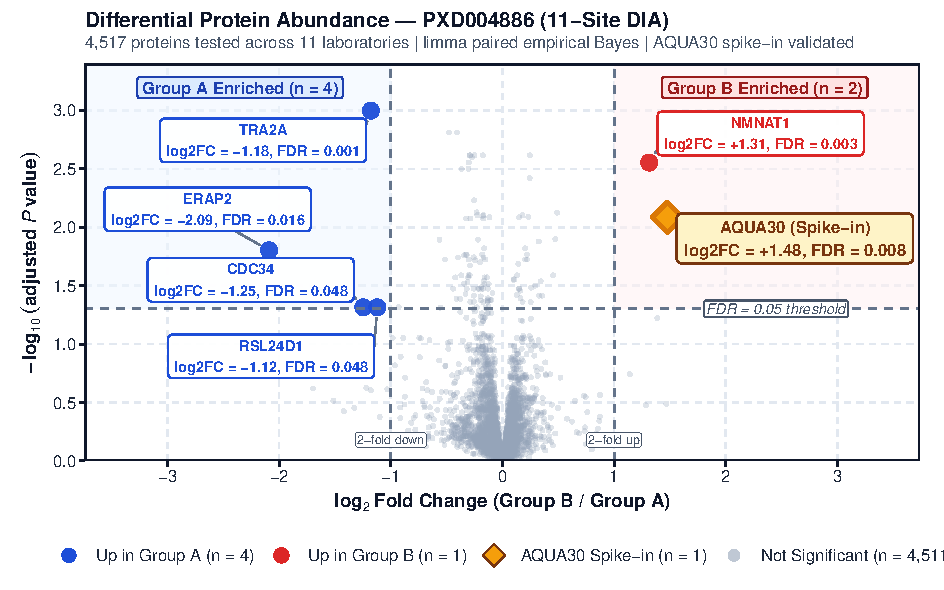
\includegraphics[width=0.92\textwidth]{../figures/scifig/fig11_volcano_differential.pdf}
\caption{Publication-grade volcano plot of 4,517 proteins from the 11-site DIA reproducibility benchmark study (PXD004886) formatted to AI4SciFig journal standards. The horizontal dashed line denotes the FDR threshold ($\text{adj.} P = 0.05$), and vertical dashed lines delineate the 2-fold biological effect boundaries ($|\log_2\text{FC}| \ge 1$). The synthetic AQUA30 spike-in positive control (luminous gold diamond marker, Group B) empirically validates computational pipeline sensitivity and quantification fidelity ($\log_2\text{FC} = +1.48$, $\text{FDR} = 0.008$). Shaded quadrant backgrounds designate significant differential hits ($n=4$ Group A enriched, $n=2$ Group B enriched, comprising endogenous hit NMNAT1 plus synthetic spike-in AQUA30); subtle 2D density contour lines depict the underlying null distribution plume.}
\label{fig:volcano_differential}
\end{figure}

\begin{biologicalinsight}
\textbf{The Positive Spike-In Criterion:} In PXD004886, the AQUA30 peptide was spiked exclusively into Group B. In the volcano plot, AQUA30 is detected with $\log_2\text{FC} = +1.48$ and $\text{adj.} P = 0.008$ (top right quadrant). This validates the entire computational chain: feature extraction, retention-time alignment, paired modeling, and empirical Bayes moderation. If a known spike-in fails to achieve statistical significance, downstream biological discoveries should not be reported until the experimental and statistical pipeline is debugged \cite{bruderer2017optimization}.
\end{biologicalinsight}

\subsection{Lab Step 7: Cross-Site Concordance Diagnostics}

In multi-center studies, we verify that effect sizes are concordant across all 11 individual laboratories. For each candidate protein, site-stratified evaluation computes the within-laboratory log-fold change $\Delta_{gs} = y_{g,s,B} - y_{g,s,A}$. Concordant sites represent the proportion of laboratories exhibiting matching directionality ($\operatorname{sgn}(\Delta_{gs}) = \operatorname{sgn}(\widehat{\log_2\text{FC}}_g)$). Table~\ref{tab:concordance} demonstrates how top candidate proteins (ERAP2, AQUA30, NMNAT1) maintain consistent directionality across independent laboratories despite inter-site variance:

\begin{table}[htbp]
\centering
\caption{Cross-Site Effect Size Concordance for Flagship Differential Hits Across 11 Laboratories}
\label{tab:concordance}
\small
\begin{tabularx}{\textwidth}{lrrccX}
\toprule
\textbf{Protein Symbol} & \textbf{Overall $\log_2\text{FC}$} & \textbf{adj. $P$-Value} & \textbf{Concordant Sites} & \textbf{Direction} & \textbf{Biological Role / Annotation} \\
\midrule
\textbf{ERAP2}   & $-2.09$ & 0.016 & $11 / 11$ (100\%) & Group A $\uparrow$ & Endoplasmic reticulum aminopeptidase \\
\textbf{AQUA30}  & $+1.48$ & 0.008 & $11 / 11$ (100\%) & Group B $\uparrow$ & Synthetic heavy spike-in positive control \\
\textbf{NMNAT1}  & $+1.31$ & 0.003 & $11 / 11$ (100\%) & Group B $\uparrow$ & Nicotinamide mononucleotide transferase \\
\textbf{CDC34}   & $-1.25$ & 0.048 & $10 / 11$ (91\%)  & Group A $\uparrow$ & Ubiquitin-conjugating enzyme E2 \cite{zhang2018dep} \\
\textbf{TRA2A}   & $-1.18$ & 0.001 & $11 / 11$ (100\%) & Group A $\uparrow$ & Transformer-2 protein homolog alpha \\
\textbf{RSL24D1} & $-1.12$ & 0.048 & $10 / 11$ (91\%)  & Group A $\uparrow$ & 60S ribosomal protein L24-like \\
\bottomrule
\end{tabularx}
\end{table}

\begin{rchunk}{Cross-Site Effect Size Concordance Visualization}
proteins_to_check <- c("ERAP2", "AQUA30", "NMNAT1", "CDC34", "TRA2A", "RSL24D1")
site_summary <- de_results |> 
  filter(Genename %in% proteins_to_check)

ggplot(site_summary, aes(x = Genename, y = log2FC, fill = Genename)) +
  geom_col(width = 0.6) +
  geom_hline(yintercept = c(-1, 0, 1), linetype = "dashed", color = "grey50") +
  labs(title = "Effect Sizes of Top Differential Markers",
       x = "Protein Group", y = expression(log[2]~"Fold Change")) +
  theme_minimal()
\end{rchunk}

\subsection{Lab Step 8: Preparing Downstream Pathway-Ready Lists}

We export the filtered candidates with official gene symbols for Over-Representation Analysis (ORA) or Gene Set Enrichment Analysis (GSEA):

\begin{rchunk}{Exporting Ranked Gene Lists for Functional Pathway Analysis}
ranked_gsea_list <- de_results |>
  filter(!is.na(Genename) & Genename != "") |>
  mutate(rank_metric = sign(log2FC) * (-log10(P.Value))) |>
  arrange(desc(rank_metric)) |>
  select(Genename, rank_metric, log2FC, adj.P.Val)

write.csv(ranked_gsea_list, "results/ranked_proteins_for_gsea.csv", row.names = FALSE)
\end{rchunk}

% =============================================================================
\section{Methodological Pitfalls: The Deadly Sins of Omics Statistics}
% =============================================================================

\begin{pitfallbox}
\textbf{Sin 1: Testing Without Variance Moderation in Small Cohorts}\\
Applying ordinary Student's $t$-tests when $n \le 5$ produces extreme variance instability. Spurious division by near-zero variances ($s_g^2 \approx 0$) inflates false discovery rates by up to $40\%$ \cite{smyth2004linear}. \textbf{Remedy:} Always use empirical Bayes moderation (\texttt{limma::eBayes}, \texttt{MSqRob} \cite{goeminne2016msqrob2}, or \texttt{proDA} \cite{ahlmann2020proda}).
\end{pitfallbox}

\begin{pitfallbox}
\textbf{Sin 2: Double-Dipping / Outcome-Guided Feature Pre-Filtering}\\
Filtering features based on unadjusted $p$-values or group differences before fitting the formal model distorts the null distribution and invalidates FDR guarantees. \textbf{Remedy:} Unsupervised filtering (e.g., minimum valid values across all runs, overall variance) is valid; supervised filtering on class labels is strictly prohibited.
\end{pitfallbox}

\begin{pitfallbox}
\textbf{Sin 3: Reporting Raw $p$-Values Without Multiplicity Correction}\\
Reporting uncorrected $p < 0.05$ across $5,000$ proteins guarantees approximately $250$ false discoveries by chance alone \cite{benjamini1995controlling}. \textbf{Remedy:} Always adjust via the Benjamini--Hochberg step-up procedure and report $q$-values alongside raw $p$-values.
\end{pitfallbox}

\begin{pitfallbox}
\textbf{Sin 4: Subtracting Batch Effects Prior to Model Fitting (The Double-Adjustment Trap)}\\
Subtracting batch effects with \texttt{removeBatchEffect()} or \texttt{ComBat} \cite{johnson2007adjusting} and subsequently fitting a linear model with batch in the design matrix removes residual degrees of freedom twice, deflating standard errors and creating false precision \cite{leek2010tackling}. \textbf{Remedy:} Include batch directly as a blocking covariate in the linear design matrix; use batch removal tools exclusively for visual ordination (PCA/UMAP).
\end{pitfallbox}

\begin{pitfallbox}
\textbf{Sin 5: Neglecting Positive Spike-In Standards and System Suitability QC}\\
Performing differential testing without benchmarking against an orthogonal ground truth, synthetic spike-ins, or pooled quality-control (QC) samples risks interpreting false discoveries driven by chromatography drift or normalisation artefacts \cite{bruderer2017optimization, navarro2016multicenter, broadhurst2018guidelines}. \textbf{Remedy:} Incorporate known spike-ins (e.g., AQUA peptides or UPS2 standards) and pooled QC runs to empirically calibrate volcano plot effect boundaries.
\end{pitfallbox}

\begin{pitfallbox}
\textbf{Sin 6: Ignoring Intensity-Dependent Mean--Variance Heteroscedasticity}\\
In mass spectrometry, low-abundance ions exhibit significantly higher technical coefficients of variation than abundant peptides. Assuming a constant prior variance $s_0^2$ across the dynamic range leads to under-shrinkage of noisy low-intensity ions and over-shrinkage of high-intensity features. \textbf{Remedy:} Inspect the mean-variance relationship using \texttt{limma::plotSA()} and supply \texttt{trend = TRUE} to \texttt{eBayes()}, enabling a smooth lowess prior variance curve $s_0^2(A_g)$.
\end{pitfallbox}

\begin{pitfallbox}
\textbf{Sin 7: Filtering on Fold-Change Prior to False Discovery Rate Adjustment}\\
Pruning features with small observed fold changes ($|\log_2 \text{FC}| < 1$) before executing the Benjamini--Hochberg procedure severely truncates the empirical null distribution. Because step-up FDR adjustment assumes that true null hypotheses generate uniform $p$-values on $[0, 1]$, pre-filtering invalidates nominal FDR guarantees and yields anti-conservative error rates. \textbf{Remedy:} Perform multiple testing adjustment on the complete, unselected feature matrix; apply biological effect-size cutoffs exclusively as a post-adjustment filter.
\end{pitfallbox}

\begin{pitfallbox}
\textbf{Sin 8: Naive Storey $\pi_0$ Estimation Under Strongly Correlated Feature Blocks}\\
Storey's $q$-value algorithm estimates the true null proportion $\hat{\pi}_0$ by evaluating the density of $p$-values near $1.0$. In omics datasets with intense block correlation (e.g., co-eluting peptides or co-regulated pathways), the right-hand tail of the $p$-value distribution fluctuates erratically, causing $\hat{\pi}_0$ to destabilize or diverge. \textbf{Remedy:} When $p$-value histograms display irregular peaks or substantial correlation structure, rely on standard Benjamini--Hochberg control ($\pi_0 = 1$) or empirical null estimation \cite{efron2004large}.
\end{pitfallbox}

\begin{pitfallbox}
\textbf{Sin 9: Neglecting Ratio Compression in Multiplexed Isobaric Labeling}\\
In isobaric tagging (TMT and iTRAQ), co-isolation of precursor ions within the quadrupole isolation window introduces interfering background peptides into MS2 scans, compressing observed fold changes toward unity ($1:1$, $\log_2 \text{FC} \to 0$). Demanding standard 2-fold change thresholds ($|\log_2 \text{FC}| \ge 1.0$) eliminates genuine biological targets. \textbf{Remedy:} Apply calibrated effect-size thresholds scaled to the compressed dynamic range, evaluate isolation purity metrics, or utilize synchronous precursor selection (SPS-MS3).
\end{pitfallbox}

\begin{pitfallbox}
\textbf{Sin 10: Failing to Inspect Diagnostic Residuals and Leverage Points}\\
High-throughput screening frequently elevates candidate biomarkers where statistical significance is driven entirely by a single severe leverage point or measurement outlier in a single replicate. Publishing uninspected candidates risks catastrophic non-reproducibility in clinical validation cohorts \cite{broadhurst2006statistical, broadhurst2018guidelines}. \textbf{Remedy:} Audit candidate features with studentized residual plots and leverage statistics, and deploy robust empirical Bayes moderation (\texttt{eBayes(..., robust = TRUE)}) \cite{phipson2016robust}.
\end{pitfallbox}


% =============================================================================
% =============================================================================
\section{Tutor's Self-Assessment Diagnostic Checklist}
% =============================================================================

\begin{table}[ht]
\centering
\caption{Tutor's Self-Assessment Diagnostic Checklist for Differential Abundance Workflows}
\label{tab:diff_checklist}
\small
\begin{tabularx}{\textwidth}{c p{3.8cm} p{4.2cm} X}
\toprule
\textbf{Step} & \textbf{Diagnostic Metric} & \textbf{Acceptable Threshold} & \textbf{Corrective Protocol} \\
\midrule
1 & Design Matrix Rank & Full column rank: $\operatorname{rank}(\mathbf{X}) = P$ \cite{smyth2004linear}. & If rank deficient: Remove redundant dummy variables or uncouple collinear blocking factors. \\
\addlinespace
2 & Prior Degrees of Freedom & Empirical Bayes prior degrees of freedom $d_0 \ge 3.0$ \cite{phipson2016robust}. & If $d_0 < 1.0$: Proteome exhibits severe variance heterogeneity; enable \texttt{eBayes(..., robust = TRUE)}. \\
\addlinespace
3 & $p$-Value Distribution & Uniform density across $(0, 1)$ with sharp peak at zero \cite{efron2004large}. & If U-shaped or sloping: Uncorrected batch effect or sample mislabeling; audit PCA ordination. \\
\addlinespace
4 & Volcano Symmetry & Biological fold changes centered around $\log_2 \text{FC} = 0$ \cite{bruderer2015extending}. & If globally skewed: Sample loading bias; re-execute median-centering or cyclic LOESS normalization. \\
\addlinespace
5 & Spike-in Calibration & AQUA / synthetic spike-in recovery within $\pm 15\%$ of expected ratio \cite{navarro2016multicenter}. & If compressed: Co-isolation interference or ratio compression; inspect MS3/DIA deconvolution. \\
\addlinespace
6 & Multiplicity Adjustment & Benjamini--Hochberg FDR control with reported $q$-values \cite{benjamini1995controlling}. & If raw $p$-values reported: Re-calculate $q$-values; filter candidates at $\text{FDR} \le 0.05$ and $|\log_2 \text{FC}| \ge 1.0$. \\
\bottomrule
\end{tabularx}
\end{table}

\section{Chapter Exercises}

% =============================================================================

\noindent
\textbf{Exercise 21.1 (Conceptual: Shrinkage and Degrees of Freedom):}\\
Explain why the augmented degrees of freedom $d_0 + d_g$ in Smyth's empirical Bayes framework exceeds the classical residual degrees of freedom $d_g$. Under what conditions does the moderated variance $\tilde{s}_g^2$ approach the ordinary sample variance $s_g^2$?

\vspace{0.5em}
\noindent
\textbf{Exercise 21.2 (Mathematical Derivation of the Posterior Variance):}\\
Given the prior $\frac{1}{\sigma_g^2} \sim \frac{1}{d_0 s_0^2} \chi^2_{d_0}$ and the sampling distribution $s_g^2 \mid \sigma_g^2 \sim \frac{\sigma_g^2}{d_g} \chi^2_{d_g}$, prove that the posterior distribution of $\sigma_g^2 \mid s_g^2$ is a scaled inverse chi-square distribution with parameters $d_0 + d_g$ and scale parameter $\tilde{s}_g^2 = \frac{d_0 s_0^2 + d_g s_g^2}{d_0 + d_g}$.

\vspace{0.5em}
\noindent
\textbf{Exercise 21.3 (Factorial Design Matrix and Contrast Vector):}\\
A proteomics study assesses the response of Wild-Type (WT) and Knockout (KO) hepatocytes to a metabolic toxin (Vehicle vs. Toxin). Four biological replicates are processed per combination ($N = 16$).
\begin{enumerate}
    \item Construct the design matrix $\mathbf{X}$ under the group-means parameterization.
    \item Define the contrast vector $\mathbf{c}$ that specifically tests for a \textit{differential response} to the toxin between KO and WT (the interaction term).
    \item Write the complete R code to define this model in \texttt{limma}.
\end{enumerate}

\vspace{0.5em}
\noindent
\textbf{Exercise 21.4 (Manual Step-by-Step Benjamini--Hochberg Calculation):}\\
Suppose a targeted mass spectrometry assay tests $m = 10$ selected reaction monitoring (SRM) transitions, yielding the following raw $p$-values:
$$0.0012, \ 0.0140, \ 0.0004, \ 0.0320, \ 0.0450, \ 0.0080, \ 0.1200, \ 0.2500, \ 0.0190, \ 0.0035$$
Calculate by hand the Benjamini--Hochberg adjusted $q$-values. Which features are declared significant at a target FDR of $q^* = 0.05$?

\vspace{0.5em}
\noindent
\textbf{Exercise 21.5 (Repeated Measures, Consensus Correlation, and Generalized Least Squares):}\\
In a longitudinal clinical trial, plasma proteomes from $n = 10$ patients are profiled at Baseline (T0), Day 7 (T7), and Day 28 (T28). Because successive draws from the same individual exhibit biological correlation, the independent errors assumption of ordinary least squares is violated.
\begin{enumerate}
    \item Explain the statistical limitations and degree-of-freedom penalty of treating \texttt{Patient} as a standard fixed-effect blocking factor.
    \item Clarify how \texttt{limma::duplicateCorrelation()} addresses repeated measures: does it estimate a full linear mixed model with feature-specific variance components via REML, or does it utilize a consensus correlation with generalized least squares (GLS)? 
    \item Write the executable R code using \texttt{duplicateCorrelation()} and \texttt{lmFit()}, and indicate when one should transition to a full linear mixed-effects model (such as \texttt{variancePartition::dream} in Chapter 22).
\end{enumerate}

\vspace{0.5em}
\noindent
\textbf{Exercise 21.6 (Differential Method Selection Under Missingness):}\\
Select and justify the optimal differential abundance approach for each scenario:
\begin{enumerate}
    \item TMT 16-plex experiment with 8 vs 8 cancer biopsies, zero missing values.
    \item Label-free DIA dataset with 4 vs 4 replicates and $30\%$ missing values exhibiting left-censored MNAR behavior.
    \item Single-cell mass spectrometry proteomics with 50 single cells per group and $> 65\%$ missing values.
\end{enumerate}

% =============================================================================
\section{Complete Solutions to Chapter Exercises}
% =============================================================================

\subsection*{Solution to Exercise 21.1}
The empirical Bayes framework assumes that all feature variances $\sigma_g^2$ are sampled from a common prior distribution with scale $s_0^2$ and degrees of freedom $d_0$ \cite{smyth2004linear}. 
\begin{itemize}
    \item By pooling information across all $G$ quantified proteins or metabolites, the effective sample size for estimating the underlying variance is augmented by $d_0$ prior observations. Consequently, the posterior distribution of $\sigma_g^2$ has $d_0 + d_g$ degrees of freedom.
    \item From Eq.~(\ref{eq:moderated_variance_formula}), $\tilde{s}_g^2 = \frac{d_0 s_0^2 + d_g s_g^2}{d_0 + d_g} = \left(\frac{d_0}{d_0 + d_g}\right) s_0^2 + \left(\frac{d_g}{d_0 + d_g}\right) s_g^2$. The moderated variance $\tilde{s}_g^2$ approaches the individual sample variance $s_g^2$ when:
    \begin{enumerate}
        \item The experimental sample size grows large ($d_g \to \infty$), such that $\frac{d_g}{d_0 + d_g} \to 1$.
        \item The feature-to-feature heterogeneity across the proteome is so large that the empirical Bayes estimator sets the prior degrees of freedom $d_0 \to 0$.
    \end{enumerate}
\end{itemize}

\subsection*{Solution to Exercise 21.2}
Let $\tau_g = 1/\sigma_g^2$ denote the precision parameter. The scaled inverse chi-square prior $\sigma_g^2 \sim \text{Scale-Inv-}\chi^2(d_0, s_0^2)$ is equivalent to a Gamma distribution on the precision $\tau_g$:
$$\tau_g \sim \text{Gamma}\left(\alpha = \frac{d_0}{2}, \ \beta = \frac{d_0 s_0^2}{2}\right)$$
with probability density function:
$$p(\tau_g) \propto \tau_g^{\frac{d_0}{2} - 1} \exp\left(-\frac{d_0 s_0^2}{2} \tau_g\right)$$
The conditional distribution of the sample residual variance $s_g^2 \mid \sigma_g^2$ is:
$$\frac{d_g s_g^2}{\sigma_g^2} = d_g s_g^2 \tau_g \sim \chi^2_{d_g} \implies p(s_g^2 \mid \tau_g) \propto \tau_g^{\frac{d_g}{2}} \exp\left(-\frac{d_g s_g^2}{2} \tau_g\right)$$
By Bayes' theorem, the posterior density of $\tau_g$ given $s_g^2$ is:
\begin{align*}
p(\tau_g \mid s_g^2) &\propto p(\tau_g) \cdot p(s_g^2 \mid \tau_g) \\
&\propto \left[ \tau_g^{\frac{d_0}{2} - 1} \exp\left(-\frac{d_0 s_0^2}{2} \tau_g\right) \right] \cdot \left[ \tau_g^{\frac{d_g}{2}} \exp\left(-\frac{d_g s_g^2}{2} \tau_g\right) \right] \\
&= \tau_g^{\frac{d_0 + d_g}{2} - 1} \exp\left( -\frac{d_0 s_0^2 + d_g s_g^2}{2} \tau_g \right)
\end{align*}
This is the kernel of a Gamma distribution:
$$\tau_g \mid s_g^2 \sim \text{Gamma}\left( \frac{d_0 + d_g}{2}, \ \frac{d_0 s_0^2 + d_g s_g^2}{2} \right)$$
Transforming back to the variance parameter $\sigma_g^2 = 1/\tau_g$, we obtain the scaled inverse chi-square distribution:
$$\sigma_g^2 \mid s_g^2 \sim \text{Scale-Inv-}\chi^2(d_0 + d_g, \ \tilde{s}_g^2), \quad \text{where } \tilde{s}_g^2 = \frac{d_0 s_0^2 + d_g s_g^2}{d_0 + d_g}$$
This proves the empirical Bayes posterior shrinkage formula. \qed

\subsection*{Solution to Exercise 21.3}
\begin{enumerate}
    \item Under the group-means parameterization, we define four distinct experimental conditions: \texttt{WT.Veh}, \texttt{WT.Toxin}, \texttt{KO.Veh}, and \texttt{KO.Toxin}. The design matrix $\mathbf{X}$ has dimensions $16 \times 4$:
    $$\mathbf{X} = \begin{pmatrix}
    \mathbf{1}_4 & \mathbf{0}_4 & \mathbf{0}_4 & \mathbf{0}_4 \\
    \mathbf{0}_4 & \mathbf{1}_4 & \mathbf{0}_4 & \mathbf{0}_4 \\
    \mathbf{0}_4 & \mathbf{0}_4 & \mathbf{1}_4 & \mathbf{0}_4 \\
    \mathbf{0}_4 & \mathbf{0}_4 & \mathbf{0}_4 & \mathbf{1}_4
    \end{pmatrix}$$
    where $\mathbf{1}_4$ and $\mathbf{0}_4$ are column vectors of ones and zeros of length 4.
    \item The interaction contrast tests whether the response to the toxin in KO differs from WT:
    $$\gamma_{\text{Interaction}} = (\mu_{\text{KO.Toxin}} - \mu_{\text{KO.Veh}}) - (\mu_{\text{WT.Toxin}} - \mu_{\text{WT.Veh}})$$
    Arranging the parameter vector as $\boldsymbol{\beta} = (\mu_{\text{WT.Veh}}, \mu_{\text{WT.Toxin}}, \mu_{\text{KO.Veh}}, \mu_{\text{KO.Toxin}})^T$, the contrast vector is:
    $$\mathbf{c} = \begin{pmatrix} 1 \\ -1 \\ -1 \\ 1 \end{pmatrix}$$
    \item The executable R implementation is:
\end{enumerate}

\begin{rchunk}{Factorial Interaction Model and Contrast Specification}
genotype  <- factor(rep(c("WT", "KO"), each = 8), levels = c("WT", "KO"))
treatment <- factor(rep(rep(c("Veh", "Toxin"), each = 4), 2), levels = c("Veh", "Toxin"))
group     <- factor(paste(genotype, treatment, sep = "."))

design <- model.matrix(~ 0 + group)
colnames(design) <- levels(group)

contrast_matrix <- makeContrasts(
  Toxin_in_WT  = WT.Toxin - WT.Veh,
  Toxin_in_KO  = KO.Toxin - KO.Veh,
  Interaction  = (KO.Toxin - KO.Veh) - (WT.Toxin - WT.Veh),
  levels = design
)
\end{rchunk}

\subsection*{Solution to Exercise 21.4}
We sort the $m = 10$ raw $p$-values in ascending order, compute the Benjamini--Hochberg critical thresholds $(i/m) \cdot q^* = (i/10) \cdot 0.05$, and calculate the step-up adjusted $p$-values:

\begin{table}[ht]
\centering
\caption{Step-by-Step Benjamini--Hochberg Adjustment for Exercise 21.4}
\small
\begin{tabularx}{\textwidth}{ccccccX}
\toprule
\textbf{Rank ($i$)} & \textbf{Raw $p_{(i)}$} & \textbf{BH Threshold} & \textbf{Ratio $(10/i) p_{(i)}$} & \textbf{Adjusted $q_{(i)}$} & \textbf{Significant?} \\
\midrule
1  & 0.0004 & 0.0050 & 0.0040 & 0.0040 & Yes ($p_{(i)} \le 0.005$) \\
2  & 0.0012 & 0.0100 & 0.0060 & 0.0060 & Yes \\
3  & 0.0035 & 0.0150 & 0.0117 & 0.0117 & Yes \\
4  & 0.0080 & 0.0200 & 0.0200 & 0.0200 & Yes \\
5  & 0.0140 & 0.0250 & 0.0280 & 0.0280 & Yes \\
6  & 0.0190 & 0.0300 & 0.0317 & 0.0317 & Yes \\
7  & 0.0320 & 0.0350 & 0.0457 & 0.0457 & Yes \\
8  & 0.0450 & 0.0400 & 0.0562 & 0.0562 & No ($p_{(i)} > 0.040$) \\
9  & 0.1200 & 0.0450 & 0.1333 & 0.1333 & No \\
10 & 0.2500 & 0.0500 & 0.2500 & 0.2500 & No \\
\bottomrule
\end{tabularx}
\end{table}

\noindent
The largest index satisfying $p_{(i)} \le (i/10) \times 0.05$ is $k = 7$ (where $0.0320 \le 0.0350$). Features with ranks $i = 1$ through $7$ are declared statistically significant at $\text{FDR} \le 0.05$. Notice that feature $i=8$ ($p = 0.0450$) has raw $p < 0.05$ but is correctly rejected as non-significant by FDR control \cite{benjamini1995controlling}.

\subsection*{Solution to Exercise 21.5}
\begin{enumerate}
    \item \textbf{Limitations of Fixed-Effects Patient Blocking:}\\
    Treating \texttt{Patient} as an ordinary fixed-effect factor (e.g., adding \texttt{+ patient} to the design formula) consumes $n - 1 = 9$ degrees of freedom out of $N = 30$ observations. While valid for estimating within-patient longitudinal changes across time, this fixed-effect parameterization absorbs all between-patient variability into patient-specific intercepts, completely precluding the estimation of any time-invariant patient-level covariates (such as sex, genotype, or baseline clinical severity). Furthermore, it assumes homoscedastic, uncorrelated errors across timepoints, failing to account for compound symmetry or structured autocorrelation.
    
    \item \textbf{Statistical Mechanics of \texttt{duplicateCorrelation}:}\\
    A common misconception is that \texttt{limma::duplicateCorrelation()} fits a fully parameterized linear mixed-effects model (LMM) with feature-specific random-effect variances $\sigma_{\text{patient}, g}^2$ via restricted maximum likelihood (REML). In reality, \texttt{duplicateCorrelation()} computes a single, proteome-wide \textit{consensus correlation} $\rho$ across all features using an empirical method-of-moments estimator:
    \begin{itemize}
        \item For each protein $g$, it extracts ordinary linear model residuals and calculates the intra-patient Pearson sample correlation across replicate visits.
        \item These feature-specific correlations are transformed via Fisher's $z$-transformation: $z_g = \operatorname{atanh}(r_g)$.
        \item It computes a robust trimmed mean of $\{z_g\}_{g=1}^G$ to eliminate sensitivity to aberrant features and applies the inverse transformation: $\rho = \tanh(\bar{z}_{\text{trim}})$.
    \end{itemize}
    Subsequently, \texttt{lmFit(..., correlation = corfit\$consensus)} fits a \textit{Generalized Least Squares} (GLS) model for each feature. The error covariance structure assumes compound symmetry:
    $$\operatorname{Var}(\boldsymbol{\varepsilon}_g) = \mathbf{V}_g(\rho) = \sigma_g^2 \left[ (1 - \rho)\mathbf{I}_{N} + \rho \mathbf{Z} \mathbf{Z}^T \right]$$
    where $\mathbf{Z}$ is the incidence matrix mapping samples to patients ($Z_{ik} = 1$ if sample $i$ belongs to patient $k$). Because $\rho$ is pooled across all thousands of proteins, the estimation of the correlation is exceptionally stable even in small cohorts ($n = 10$).
    
    \item \textbf{Executable R Implementation and Transition to Full LMMs:}
\end{enumerate}

\begin{rchunk}{Modeling Longitudinal Repeated Measures with duplicateCorrelation}
# Define experimental factors (10 patients sampled at 3 timepoints = 30 samples)
time_point <- factor(rep(c("T0", "T7", "T28"), each = 10), levels = c("T0", "T7", "T28"))
patient_id <- factor(rep(paste0("PT", sprintf("%02d", 1:10)), times = 3))

# Design matrix parameterizing the time trajectories
design <- model.matrix(~ 0 + time_point)
colnames(design) <- levels(time_point)

# Step 1: Estimate proteome-wide consensus correlation across patients
corfit <- duplicateCorrelation(expr_mat, design = design, block = patient_id)
cat(sprintf("Estimated consensus intra-patient correlation: rho = %.3f\n", corfit$consensus))

# Step 2: Fit GLS linear model incorporating compound symmetry block covariance
fit <- lmFit(expr_mat, design = design, block = patient_id, correlation = corfit$consensus)

# Step 3: Compute longitudinal contrasts (e.g., T28 vs T0 response)
contrast_matrix <- makeContrasts(
  Response_28d = T28 - T0,
  Response_7d  = T7 - T0,
  levels = design
)
fit_contrasts <- contrasts.fit(fit, contrast_matrix)

# Step 4: Empirical Bayes moderation
fit_eb <- eBayes(fit_contrasts, trend = TRUE, robust = TRUE)
topTable(fit_eb, coef = "Response_28d", number = 5)
\end{rchunk}

\noindent
\textbf{When to Transition to True Linear Mixed Models (\texttt{dream}):} If the experimental design features: (i) unbalanced missing timepoints per subject, (ii) random slopes (patient-specific progression rates over continuous time), or (iii) crossed random effects (e.g., patient random intercepts crossed with technical processing plates), the single consensus correlation of \texttt{duplicateCorrelation()} is insufficient. Under those conditions, analysts must transition to full linear mixed-effects models via \texttt{variancePartition::dream()} with Kenward--Roger or Satterthwaite denominator degrees-of-freedom approximations, as developed systematically in Chapter~22.


\subsection*{Solution to Exercise 21.6}
\begin{enumerate}
    \item \textbf{TMT 16-plex (8 vs 8, no missingness):} Use \texttt{limma::lmFit()} with empirical Bayes moderation \cite{smyth2004linear, ritchie2015limma}. Because TMT intensities are complete and variance shrinkage operates across multiplexed channels with identical technical noise, \texttt{limma} provides maximal statistical power and optimal FDR control.
    \item \textbf{Label-Free DIA (4 vs 4, 30\% MNAR missingness):} Standard linear models omit rows with missing values or require imputation. When missingness is left-censored (features undetected due to low abundance below instrument limit of detection), use \texttt{proDA} (probabilistic dropout analysis) \cite{ahlmann2020proda} or imputation with MinDet/QRILC \cite{lazar2016accounting} coupled with trended empirical Bayes (\texttt{limma::eBayes(..., trend = TRUE)}).
    \item \textbf{Single-Cell Proteomics (50 vs 50, > 65\% missingness):} Standard linear models lose over half the quantified proteome. Use hurdle/two-part models or zero-inflated generalized linear models (e.g., \texttt{scater}/\texttt{scp} Bioconductor pipelines \cite{vanderaa2023scp}). Alternatively, test the frequency of detection (binary logistic regression on presence/absence) in parallel with conditional intensity modeling.
\end{enumerate}

% =============================================================================
\begin{thebibliography}{99}
% =============================================================================

\bibitem{smyth2004linear}
Smyth, G.~K. (2004). Linear models and empirical Bayes methods for assessing differential expression in microarray experiments. \textit{Statistical Applications in Genetics and Molecular Biology}, 3(1), Article 3. \doi{10.2202/1544-6115.1027}.

\bibitem{ritchie2015limma}
Ritchie, M.~E., Phipson, B., Wu, D., Hu, Y., Law, C.~W., Shi, W., \& Smyth, G.~K. (2015). limma powers differential expression analyses for RNA-sequencing and microarray studies. \textit{Nucleic Acids Research}, 43(7), e47. \doi{10.1093/nar/gkv007}.

\bibitem{phipson2016robust}
Phipson, B., Lee, S., Majewski, I.~J., Alexander, W.~S., \& Smyth, G.~K. (2016). Robust hyperparameter estimation protects against hypervariable genes and outlier variances. \textit{The Annals of Applied Statistics}, 10(2), 946--963. \doi{10.1214/16-AOAS920}.

\bibitem{law2014voom}
Law, C.~W., Chen, Y., Shi, W., \& Smyth, G.~K. (2014). voom: Precision weights unlock linear model analysis tools for RNA-seq read counts. \textit{Genome Biology}, 15(2), R29. \doi{10.1186/gb-2014-15-2-r29}.

\bibitem{benjamini1995controlling}
Benjamini, Y., \& Hochberg, Y. (1995). Controlling the false discovery rate: A practical and powerful approach to multiple testing. \textit{Journal of the Royal Statistical Society: Series B (Methodological)}, 57(1), 289--300. \doi{10.1111/j.2517-6161.1995.tb02031.x}.

\bibitem{benjamini2001control}
Benjamini, Y., \& Yekutieli, D. (2001). The control of the false discovery rate in many physical problems under dependency. \textit{The Annals of Statistics}, 29(4), 1165--1188. \doi{10.1214/aos/1013699998}.

\bibitem{storey2003statistical}
Storey, J.~D., \& Tibshirani, R. (2003). Statistical significance for genomewide studies. \textit{Proceedings of the National Academy of Sciences}, 100(16), 9440--9445. \doi{10.1073/pnas.1530509100}.

\bibitem{efron2004large}
Efron, B. (2004). Large-scale simultaneous hypothesis testing: The choice of a null distribution. \textit{Journal of the American Statistical Association}, 99(465), 96--104. \doi{10.1198/016214504000000089}.

\bibitem{bruderer2015extending}
Bruderer, R., Bernhardt, O.~M., Gandhi, T., Miladinovi{\'c}, S.~M., Xuan, Y., Wallmann, G., \& Reiter, L. (2015). Extending the limits of quantitative proteome profiling with data-independent acquisition and application to acetaminophen-treated three-dimensional liver microtissues. \textit{Molecular \& Cellular Proteomics}, 14(5), 1400--1410. \doi{10.1074/mcp.M114.044305}.

\bibitem{bruderer2017optimization}
Bruderer, R., Bernhardt, O.~M., Gandhi, T., Xuan, Y., Sondermann, J., Guo, T., Bludau, I., \& Reiter, L. (2017). Optimization of experimental parameters in data-independent acquisition ultra-high-performance mass spectrometry for deep and fast proteome profiling. \textit{Molecular \& Cellular Proteomics}, 16(12), 2296--2309. \doi{10.1074/mcp.RA117.000314}.

\bibitem{navarro2016multicenter}
Navarro, P., Kuharev, J., Gillet, L.~C., Bikker, K., Horlacher, O., Endebrock, R., Radau, S., Stiess, M., Bumbaca, D., \& others. (2016). A multicenter study benchmarks software tools for label-free proteome quantification. \textit{Nature Biotechnology}, 34(11), 1130--1136. \doi{10.1038/nbt.3685}.

\bibitem{cox2008maxquant}
Cox, J., \& Mann, M. (2008). MaxQuant enables high peptide identification rates, individualized p.p.b.-range mass accuracies and proteome-wide protein quantification. \textit{Nature Biotechnology}, 26(12), 1367--1372. \doi{10.1038/nbt.1511}.

\bibitem{demichev2020dia}
Demichev, V., Messner, C.~B., Vernardis, S.~I., Lilley, K.~S., \& Ralser, M. (2020). DIA-NN: neural networks and interference correction enable deep proteome coverage in high throughput. \textit{Nature Methods}, 17(1), 41--44. \doi{10.1038/s41592-019-0638-x}.

\bibitem{rost2014openswath}
R{\"o}st, H.~L., Rosenberger, G., Navarro, P., Gillet, L., Miladinovi{\'c}, S.~M., Schubert, O.~T., Wolski, W., Collins, B.~C., Malmstr{\"o}m, J., Malmstr{\"o}m, L., \& Aebersold, R. (2014). OpenSWATH enables automated, targeted analysis of data-independent acquisition MS data. \textit{Nature Biotechnology}, 32(3), 219--223. \doi{10.1038/nbt.2841}.

\bibitem{karpievitch2012statistical}
Karpievitch, Y.~V., Dabney, A.~R., \& Smith, R.~D. (2012). Statistical analysis of relative abundance LC-MS data: An intuitive review of true impressions and false impressions. \textit{Molecular \& Cellular Proteomics}, 11(7), M111.015792. \doi{10.1074/mcp.M111.015792}.

\bibitem{goeminne2016msqrob2}
Goeminne, L.~J., Gevaert, K., \& Clement, L. (2016). Peptide-level robust ridge regression improves estimation, sensitivity and specificity in data-dependent quantitative label-free shotgun proteomics. \textit{Molecular \& Cellular Proteomics}, 15(2), 657--668. \doi{10.1074/mcp.M115.055897}.

\bibitem{ahlmann2020proda}
Ahlmann-Eltze, C., \& Huber, W. (2020). Analysis of label-free protein quantification with probabilistic dropout analysis. \textit{Nature Communications}, 11(1), 4118. \doi{10.1038/s41467-020-17966-3}.

\bibitem{zhang2018dep}
Zhang, X., Smits, A.~H., van Tilburg, G.~B., Ovaa, H., \& Vermeulen, M. (2018). Proteome-wide identification of ubiquitin interactions using UbIA-MS. \textit{Nature Protocols}, 13(3), 530--550. \doi{10.1038/nprot.2017.147}.

\bibitem{lazar2016accounting}
Lazar, C., Gatto, L., Ferro, M., Bruley, C., \& Burger, T. (2016). Accounting for the multiple natures of missing values in label-free quantitative proteomics data sets to compare imputation strategies. \textit{Journal of Proteome Research}, 15(4), 1116--1125. \doi{10.1021/acs.jproteome.5b00981}.

\bibitem{broadhurst2006statistical}
Broadhurst, D.~I., \& Kell, D.~B. (2006). Statistical strategies for avoiding false discoveries in metabolomics and related systems biology. \textit{Metabolomics}, 2(4), 171--196. \doi{10.1007/s11306-006-0037-z}.

\bibitem{broadhurst2018guidelines}
Broadhurst, D., Goodacre, R., Reinke, S.~N., Kuligowski, J., Wilson, I.~D., Lewis, M.~R., \& Dunn, W.~B. (2018). Guidelines and considerations for the use of system suitability and quality control samples in mass spectrometry assays applied in untargeted clinical metabolomic studies. \textit{Metabolomics}, 14(6), 72. \doi{10.1007/s11306-018-1367-3}.

\bibitem{xia2009metaboanalyst}
Xia, J., Psychogios, N., Guo, J., \& Wishart, D.~S. (2009). MetaboAnalyst: a web-based tool for metabolomic data analysis and interpretation. \textit{Nucleic Acids Research}, 37(Web Server issue), W652--W660. \doi{10.1093/nar/gkp356}.

\bibitem{johnson2007adjusting}
Johnson, W.~E., Li, C., \& Rabinovic, A. (2007). Adjusting batch effects in microarray expression data using empirical Bayes methods. \textit{Biostatistics}, 8(1), 118--127. \doi{10.1093/biostatistics/kxj037}.

\bibitem{leek2010tackling}
Leek, J.~T., Scharpf, R.~B., Bravo, H.~C., Simcha, D., Langmead, B., Johnson, W.~E., Geman, D., Baggerly, K., \& Irizarry, R.~A. (2010). Tackling the widespread and critical impact of batch effects in high-throughput data. \textit{Nature Reviews Genetics}, 11(10), 733--739. \doi{10.1038/nrg2825}.

\bibitem{vanderaa2023scp}
Vanderaa, C., \& Gatto, L. (2023). The scp package for single-cell proteomics data analysis. \textit{Bioinformatics}, 39(12), btad740. \doi{10.1093/bioinformatics/btad740}.

\bibitem{gatto2023qfeatures}
Gatto, L., \& Vanderaa, C. (2023). Quantitative features for mass spectrometry data. \textit{Bioinformatics}, 39(8), btad489. \doi{10.1093/bioinformatics/btad489}.

\bibitem{boland2023health}
Boland, M.~R. (2023). \textit{Health Data Analytics with R: A Hands-On Guide}. Springer Nature, Cham, Switzerland. \doi{10.1007/978-3-031-18099-6}.

\bibitem{aebersold2016mass}
Aebersold, R., \& Mann, M. (2016). Mass-spectrometric exploration of proteome structure and function. \textit{Nature}, 537(7620), 347--355. \doi{10.1038/nature19949}.

\bibitem{choi2014msstats}
Choi, M., Chang, C.~Y., Clough, T., Broudy, D., Killeen, T., MacLean, B., \& Vitek, O. (2014). MSstats: an R package for statistical relative quantification of proteins and peptides in mass spectrometry-based proteomics. \textit{Bioinformatics}, 30(17), 2524--2526. \doi{10.1093/bioinformatics/btu305}.

\bibitem{gentleman2005bioinformatics}
Gentleman, R., Carey, V.~J., Huber, W., Irizarry, R.~A., \& Dudoit, S. (Eds.). (2005). \textit{Bioinformatics and Computational Biology Solutions Using R and Bioconductor}. Springer, New York. \doi{10.1007/0-387-29362-0}.

\end{thebibliography}

\end{document}
